\chapter{UML Use Case Diagram} \label{ch:procedure}

\section{Diagram 1: Use Case Diagram for Multi-Tenant E-commerce System}

\subsection{Use Case Scenario 1: Vendor Registration to Create New Store}

\textbf{Use Case Name:} Register to Create New Store

\textbf{Actor:} Vendor (Small Business Owner)

\textbf{Scenario / Description:}
\begin{enumerate}
    \item Vendor navigates to the registration page.
    \item Vendor enters personal details (name, email, phone number).
    \item Vendor enters business details (store name, business type, address).
    \item Vendor creates a username and password.
    \item Vendor accepts terms and conditions.
    \item System validates all entered information.
    \item System creates a new tenant account and store database.
    \item System sends a verification email to the vendor.
    \item Vendor verifies email by clicking the confirmation link.
    \item System activates the vendor's store account.
\end{enumerate}

\textbf{Exception:}
\begin{enumerate}
    \item Email address already exists in the system.
    \item Required fields are left empty.
    \item Password does not meet security requirements.
    \item Email verification link expires before confirmation.
    \item Database connection failure during account creation.
\end{enumerate}

\textbf{Precondition:}
\begin{enumerate}
    \item Vendor has access to the registration page via web browser.
    \item Vendor has a valid email address.
    \item System database is operational.
\end{enumerate}

\textbf{Post Condition:}
\begin{enumerate}
    \item \textbf{Successful registration:} New vendor store is created in the system; vendor receives confirmation email; vendor can now log in to their store dashboard.
    \item \textbf{Unsuccessful registration:} Account is not created; system displays appropriate error messages; vendor remains on registration page to correct errors.
    \item \textbf{Exception:} Transaction is rolled back; system displays error message; vendor remains on registration page if possible.
\end{enumerate}


\subsection{Use Case Scenario 2: Vendor Login to System}

\textbf{Use Case Name:} Login to System

\textbf{Actor:} Vendor / Admin / Customer

\textbf{Scenario / Description:}
\begin{enumerate}
    \item User navigates to the login page.
    \item User enters username/email and password.
    \item User optionally selects "Remember Me" checkbox.
    \item System validates the entered credentials.
    \item System checks user role (Vendor, Admin, or Customer).
    \item System authenticates the user against the database.
    \item System creates a session for the authenticated user.
    \item System saves login information in cookies (if "Remember Me" selected).
    \item System redirects user to their respective dashboard.
\end{enumerate}

\textbf{Exception:}
\begin{enumerate}
    \item Invalid username or password entered.
    \item Account is not yet verified (pending email confirmation).
    \item Account has been suspended or deactivated.
    \item Too many failed login attempts (temporary lockout).
    \item Database connection failure during authentication.
    \item Required login page not found (404 error).
\end{enumerate}

\textbf{Precondition:}
\begin{enumerate}
    \item User has a registered account in the system.
    \item User has access to the login page URL via web browser.
    \item System database is operational and accessible.
\end{enumerate}

\textbf{Post Condition:}
\begin{enumerate}
    \item \textbf{Successful login:} User is authenticated; session is created; user is redirected to their role-specific dashboard (Vendor store dashboard, Admin panel, or Customer profile page).
    \item \textbf{Unsuccessful login:} User remains on login page; system displays appropriate error message (e.g., "Invalid username or password").
    \item \textbf{Exception:} User remains on login page if possible; system displays technical error message or redirects to error page.
\end{enumerate}

\begin{figure}[H]
    \centering
    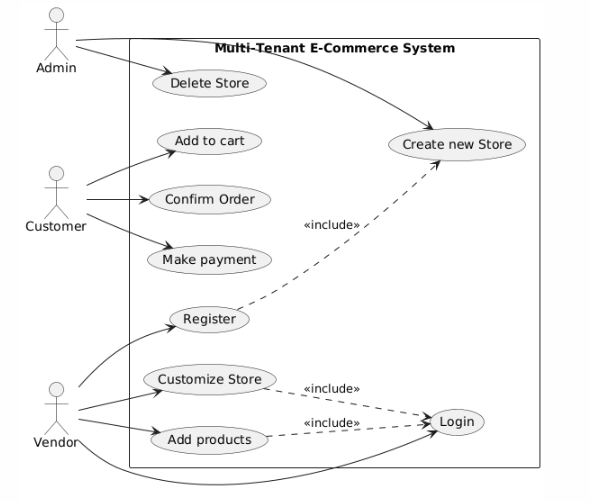
\includegraphics[width=1\linewidth]{figures/common use case uml.png}
    \caption{Multi-Tenant E-Commerce System Project UML Use case diagram}
    \label{fig:placeholder}
\end{figure}


\subsubsection*{Description}

This use case diagram provides a bird's-eye view of the entire Multi-Tenant E-Commerce System, illustrating the primary actors and their core interactions with the system. The diagram identifies three key actors: \textbf{Admin}, \textbf{Vendor}, and \textbf{Customer}.

\begin{itemize}
    \item \textbf{Admin:} The system administrator is responsible for overarching governance. The diagram shows the Admin actor connected to two key use cases: \textit{Delete Store} (to remove inappropriate or inactive vendor stores) and \textit{Login} (to access the admin panel). This actor represents the platform owner's operational control.
    
    \item \textbf{Vendor:} The small business owner (tenant) is the central user of the system. The diagram depicts the Vendor's core responsibilities, which include: \textit{Register} (to create their tenant account), \textit{Login} (to access their dashboard), \textit{Add Products} (to populate their inventory), and \textit{Customize Store} (to personalize their storefront's look and feel).
    
    \item \textbf{Customer:} The end-user who purchases products. The diagram shows the Customer's essential shopping journey: \textit{Register} (to create an account), \textit{Login} (to access their profile), \textit{Add to Cart} (to select items), \textit{Confirm Order} (to review and place the order), and \textit{Make Payment} (to complete the transaction).
\end{itemize}

This high-level diagram effectively communicates the system's boundaries and the distinct roles of each user type, serving as an excellent starting point for stakeholder discussions and scope validation.

\section{Diagram 2: Vendor-Specific Use Case Diagram (Offers \& Store Customization)}

\subsection{Use Case Scenario 3: Create Percentage Discount with Deadline}

\textbf{Use Case Name:} Create Percentage Discount with Deadline

\textbf{Actor:} Vendor

\textbf{Scenario / Description:}
\begin{enumerate}
    \item Vendor logs into their store dashboard.
    \item Vendor navigates to "Offers \& Promotions" section.
    \item Vendor selects "Create New Offer" and chooses "Percentage Discount."
    \item Vendor enters discount details:
    \begin{enumerate}
        \item Discount percentage (e.g., 10\%, 20\%, 50\%)
        \item Products or categories to apply discount to
        \item Minimum purchase amount (if applicable)
    \end{enumerate}
    \item System enforces \texttt{\textless\textless include\textgreater\textgreater} relationship: Vendor must set an offer deadline.
    \item Vendor selects offer start date and end date (deadline).
    \item System validates that end date is after start date and not in the past.
    \item Vendor optionally sets a coupon limit (maximum number of redemptions).
    \item Vendor reviews and confirms the discount offer details.
    \item System saves the discount offer and activates it according to the schedule.
    \item System displays the new offer in the vendor's active promotions list.
\end{enumerate}

\textbf{Exception:}
\begin{enumerate}
    \item Deadline (end date) is not set (violates mandatory \texttt{\textless\textless include\textgreater\textgreater} requirement).
    \item End date is earlier than start date.
    \item Start date or end date is in the past.
    \item Discount percentage is invalid (e.g., negative, zero, or >100\%).
    \item No products or categories selected for the discount.
    \item Coupon limit is set to an invalid value (negative or zero when required).
    \item Database connection failure during offer creation.
\end{enumerate}

\textbf{Precondition:}
\begin{enumerate}
    \item Vendor is logged into the system with valid session.
    \item Vendor has products listed in their inventory.
    \item System database is operational.
\end{enumerate}

\textbf{Post Condition:}
\begin{enumerate}
    \item \textbf{Successful discount creation:} New percentage discount offer is created and saved in the system; offer is scheduled according to start/end dates; customers can now avail the discount on eligible products; offer appears in vendor's promotions list.
    \item \textbf{Unsuccessful discount creation:} Discount offer is not saved; system displays appropriate error messages (e.g., "Deadline must be set," "End date must be after start date"); vendor remains on offer creation page to correct errors.
    \item \textbf{Exception:} Transaction is rolled back; system displays error message; vendor remains on offer creation page if possible.
\end{enumerate}

\begin{figure}[H]
    \centering
    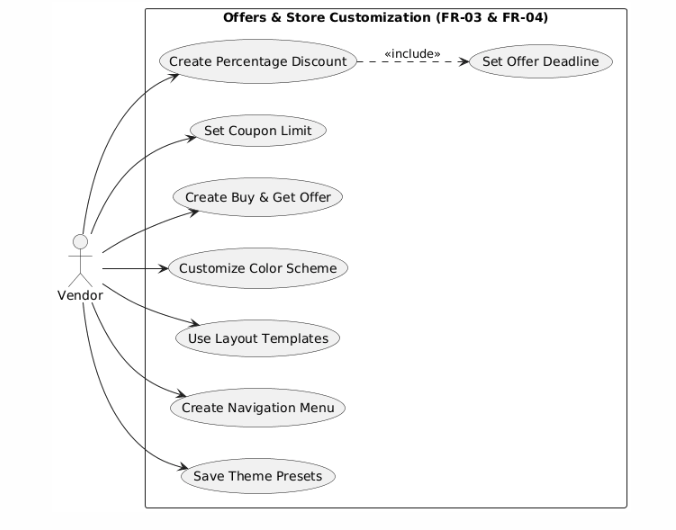
\includegraphics[width=1\linewidth]{figures/Extended usecase.png}
    \caption{Vendor specific customization and discount offers' UML Use case diagram}
    \label{fig:placeholder}
\end{figure}

\subsubsection*{Description}

This use case diagram provides a detailed, zoomed-in view of two critical vendor functionalities: \textbf{Offer Management} and \textbf{Store Customization}. It focuses exclusively on the \textbf{Vendor} actor and elaborates on the high-level "Customize Store" and implied "Manage Offers" use cases from the first diagram.

\paragraph{Offer Management Functionalities:}
The diagram shows the Vendor can create two types of offers:

\begin{itemize}
    \item \textbf{Create Percentage Discount:} To create this offer, the vendor must also \texttt{\textless\textless include\textgreater\textgreater} \textit{Set Offer Deadline}, indicating that setting a deadline is a mandatory, non-optional part of creating a percentage discount. Additionally, the vendor may optionally \textit{Set Coupon Limit}, which is shown as a separate, optional use case (extend/include relationships clarified in text).
    
    \item \textbf{Create Buy \& Get Offer:} This represents a different type of promotional offer (e.g., "Buy 1 Get 1 Free"), distinct from a simple percentage discount.
\end{itemize}

\paragraph{Store Customization Functionalities:}
The diagram details the various ways a vendor can personalize their digital storefront:

\begin{itemize}
    \item \textbf{Customize Color Scheme:} Allows the vendor to change the visual appearance.
    
    \item \textbf{Use Layout Templates:} Provides pre-designed store layouts that the vendor can apply.
    
    \item \textbf{Create Navigation Menu:} Enables the vendor to structure their store's pages and categories for easy customer browsing.
    
    \item \textbf{Save Theme Presets:} Allows the vendor to save their customization choices as reusable themes for future use.
\end{itemize}

\noindent This detailed diagram is crucial for the development team. It clarifies complex business rules (e.g., deadlines being mandatory for discounts) and ensures that all vendor-facing features are captured before database and UI design begins.

